\documentclass[9pt]{memoir}
\usepackage{multicol}
\usepackage[margin=2cm,a4paper]{geometry}
\pagestyle{empty}
\usepackage[utf8]{inputenc}
\usepackage{mathpazo}

\usepackage{graphicx}

\usepackage{tikz}
\usetikzlibrary{chains}
\usetikzlibrary{decorations}
\input{vc.tex}
\tikzstyle{whitebox} =
[     rectangle,
      inner sep = 8pt,
       fill = white,
       rounded corners,
       draw= none,
      text = black!90,
      font = \small
]
\tikzstyle{orangebox}=[
      rectangle,
      inner sep = 8pt,
      very thick,rounded corners,
      draw=white,
      fill = orange,
      text width = 7.8cm,
      text = white,
      font = \small
      ]
\begin{document}

\begin{tikzpicture}[remember picture, overlay]
  \draw [rounded corners, fill=black!10, draw=white]  
  ([xshift = +1cm,yshift = +1.3cm] current page.south west) 
  rectangle
  ([xshift = -1cm,yshift = -1cm] current page.north east);

\end{tikzpicture}

 {\fontsize{80}{110}\selectfont\textsc{CONGRESS}}

\bigskip
  {\GITAuthorName,
    rev. \GITAbrHash, \GITAuthorDate}

\begin{multicols}{2}
\textit{U.S. Congress Apportion. }
  The members of the U.S.
  Congress represent the states.
  There are more seats than states, in fact, there are 435 and 50
  states, so many states receive more than one seat in Congress.
  This is how it should be: California has 33,930,798 residents while
  Wyoming has only 495,304, so California ought to receive many more
  seats.
  On the other hand, even though California has almost 70 times as
  many residents, it would be absurd if it had 70 times as many seats
  as Wyoming.

\bigskip
\textit{Huntingdon--Hill.}
Here’s how it’s done, using the Huntingdon–Hill method from 1911:
First, each state receives a seat. (In fact, Article 1, Section 2 of
the U.S. Constitution requires that.) Then, as long as there are seats
left, we repeat the following: Give the next seat to the largest
state, and decrease the state’s population by a certain constant. The
exact procedure, including the formula for the constant, can be found
among the links below.

\bigskip
\noindent
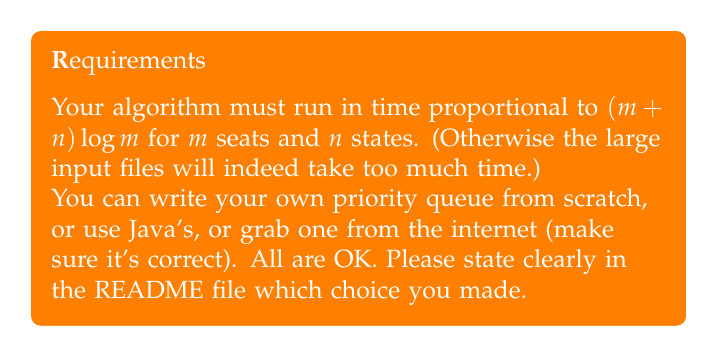
\begin{tikzpicture}
\node [orangebox]
{ {\textbf Requirements } \par\medskip\noindent
  
  Your algorithm must run in time proportional to  $(m+n) \log m$ for
  $m$ seats and $n$ states.
  (Otherwise the large input files will indeed take too much time.)
  
  You can write your own priority queue from scratch, or use Java’s,
  or grab one from the internet (make sure it’s correct).
  All are OK.
  Please state clearly in the README file which choice you made.
};
\end{tikzpicture}

\bigskip
\noindent
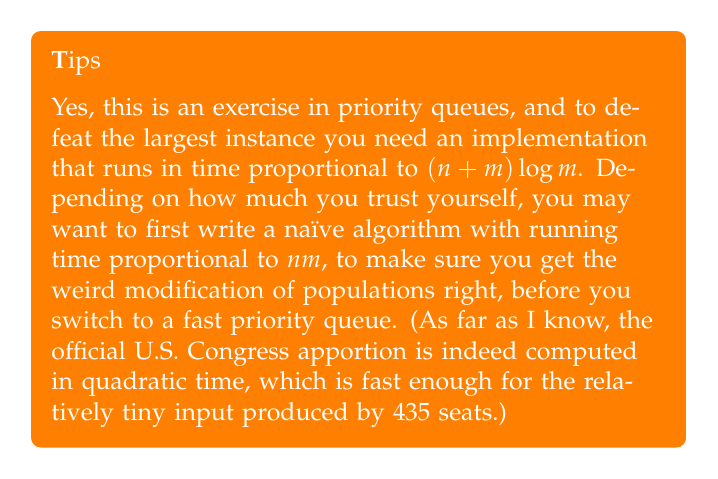
\begin{tikzpicture}
\node [orangebox] {
  {\textbf Tips }\par\medskip\noindent
  
  Yes, this is an exercise in priority queues, and to defeat the
  largest instance you need an implementation that runs in time
  proportional to $(n+m) \log m$.
  Depending on how much you trust yourself, you may want to first
  write a naïve algorithm with running time proportional to $nm$, to
  make sure you get the weird modification of populations right,
  before you switch to a fast priority queue.
  (As far as I know, the official U.S.\ Congress apportion is indeed
  computed in quadratic time, which is fast enough for the relatively
  tiny input produced by 435 seats.)
};
\end{tikzpicture}

\noindent
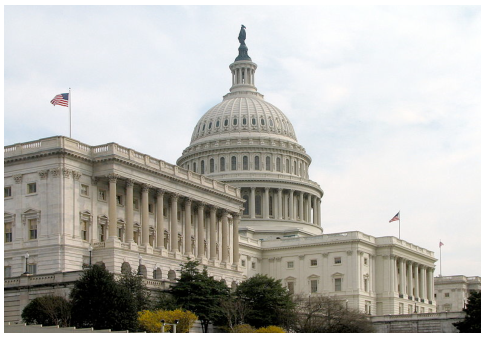
\includegraphics[width=\columnwidth]{congressphoto.pdf}



\end{multicols}

\noindent
\emph{About the files.}
The files \texttt{1990.in} and \texttt{2000.in} contain the real-world data
for the 1990 and 2000 U.S.\ censuses.
The corresponding output files are the actual seats computed in the
106th and 108th congresses.
The other files I made up.
Files called \texttt{small-*.in} are small instances that are useful for
debugging, they are meant to make your life easier.
The files called \texttt{huge-*.in} are fictional population data for
planets, the largest of these distributes the 1 million seats in the
galactic senate among 200,000 planets.
(I had fun with this.
The names of the planets are created by an algorithm similar to what
was used in the 1984 computer game Elite, picking random digrams from
``..LEXEGEZACEBISOUSESARMAINDIREA.ERATENBERALAVETIEDORQUANTEISRION''.)


\tikzstyle{listing} = [font =\ttfamily,right]
\tikzstyle{every pin} = [red, font = \itshape]
\tikzstyle{every pin edge} = [<-,red]

\begin{multicols}{2}
  \noindent
  \begin{tikzpicture}
    \matrix[fill = white]
    {
      \node [font = \itshape, right] {input file format:}; \\[1ex]
      \node [listing, pin = right:number of states] {2}; \\
      \node [listing, pin = right:number of seats] {4};\\
      \node [listing, pin = right:name of 1st state] {Gondor};\\
      \node [listing, pin = right:population of 1st state] {100};\\
      \node [listing, pin = right:name of 2nd state] {West Rohan};\\
      \node [listing, pin = right:population of 2nd state] {10};\\
    };
  \end{tikzpicture}

  \noindent
  \begin{tikzpicture}[fill = white, node distance=0pt]
    \matrix[fill=white]
    {
      \node [font = \itshape, right] {output format:}; \\[1ex]
      \node  [font = \itshape, right, red] {(lines can be in any order)}; \\[1ex]
      \node [listing, pin = left:state name, pin = right:number of
      seats] {West Rohan 1}; \\
      \node [listing] (a) {Gondor};    \\
    };
      \node (b) [base right = of a, xshift = -6pt,red,
       pin = below:separated by single space,
      ] {\textvisiblespace};
      \node (b) [base right = of b, font = \ttfamily, xshift = -6pt] {3};
  \end{tikzpicture}
  
\end{multicols}

\noindent
{\scshape References}\par\medskip

\begin{enumerate}
 \item ``United States congressional apportionment.'' \emph{Wikipedia:
     The Free Encyclopedia.}
 \item ``Huntington--Hill method.'' \emph{Wikipedia: The Free
     Encyclopedia.}
 \item Congressional apportionment, online resources maintained by the
   U.S.
   Census Bureau.\\
   www.census.gov/population/apportionment/.
\item ``Oolite planet list.'' \emph{Elite Wiki.} wiki.alioth.net/index.php/Oolite\_planet\_list.
\end{enumerate}


\end{document}